\documentclass[10pt,letterpaper]{article}

\usepackage{pslatex}
\usepackage{apacite}
\usepackage[utf8]{inputenc}
\usepackage[T1]{fontenc}
\usepackage{lmodern}
\usepackage{multicol}
\usepackage{amsmath}
\usepackage{amssymb}
\usepackage{enumitem}
\numberwithin{equation}{section}
\usepackage{algorithm}
\usepackage{algorithmic}
\usepackage{graphicx}
\usepackage{float}
\usepackage{moreverb}
\usepackage{url}
\usepackage{subcaption}
\setlength\parindent{0pt}
\usepackage{bbm}
\usepackage{booktabs}
\usepackage{longtable}
\usepackage{array}
\usepackage{multirow}
\usepackage[table]{xcolor}
\usepackage{wrapfig}
\usepackage{colortbl}
\usepackage{pdflscape}
\usepackage{tabu}
\usepackage{threeparttable}
\usepackage{threeparttablex}
\usepackage[normalem]{ulem}
\usepackage{makecell}
\usepackage{breakcites}
\usepackage[htt]{hyphenat}
\usepackage{fancyvrb}
\usepackage{algorithm}
\usepackage{algorithmic}
\usepackage{listingsutf8}
\usepackage{color}
\usepackage[margin=1in]{geometry}
\usepackage{hyperref}
\usepackage{natbib}
\usepackage[compact]{titlesec}
\titlespacing{\section}{2pt}{*2}{*1}
\titlespacing{\subsection}{2pt}{*1}{*2}
\titlespacing{\subsubsection}{0pt}{*0}{*0}

\title{{\huge \bf Semantic segmentation for learning hockey broadcast image representation}}
 
\author{{\bf Philippe Blouin-Leclerc and Stéphane Caron} \\ {Laval University} \\
{\{philippe.blouin-leclerc.1, stephane.caron.9\}}@ulaval.ca}
  
\date{May 10th 2019}

\begin{document}
\maketitle

\begin{multicols}{2}

\begin{abstract}
In this project, we propose a novel way to recognize key locations within hockey broadcast images using semantic segmentation and convolutional neural networks (CNN). The semantic representation of an image could then be used for many applications such as mapping a broadcast image into a 2D plan.  All the codes that aimed to realized that project and that article are hosted on that GitHub \href{https://github.com/stecaron/glo-7030-projet}{repository}.
\end{abstract}


\section{Introduction}
\textbf{\label{sec:introduction}}
Computer vision is a growing field that changed the faces of many applications in robotic, security or even health sectors. Another field that is currently having more and more interests in such computer vision applications is the sports analytics. The professionnal sports clubs are using analytics and data to understand as more as they can the game and the performances of their players and their opponents. To increase that understanding, you often need a bunch of experts analyzing a bunch of data. Computer vision is well suited to extract that data because it allows the detection of many events simultaneously, which otherwise may have been done by many humans. In order to extract that data properly, it's way more interesting to map those events on the field (or the ice). To do so, it's often necessary to understand the general representation of the moment (or the image), which could be done by a computer vision task called semantic segmentation.
\\
In his work, \cite{Homayounfar} present a methodology where he uses different cues on the field such as lines, corners, circles and so on to train another model that position the field in a 2 dimensionnal plan. In our project, we tried to improve the cues detection technic by training different semantic segmentation models and gain insights on how to train such models. The next step following that project will be to also use that representation in order to map players into a 2 dimensionnal plan.
\\
In the next section, we will start by giving some background about the task of semantic segmentation (section \ref{sec:background}), then we'll present our methodology (section \ref{sec:methodology}), the dataset we used for our experiments (section \ref{sec:dataset}), the results we had (section \ref{sec:results}) and finally a short conclusion (section \ref{sec:conclusion}).

 


\section{Background}
\textbf{\label{sec:background}}
\subsection{Define the task}
Before getting into more details in the \ref{sec:methodology} section, let's first define the task we will try to learn in this project. Semantic segmentation is a computer vision task where the model learns the general representation of an image by attributing a label to each and every pixels. Intuitively, to make pixel-wise predictions, you first need to have attributed a class to each pixel in the image (see figure \ref{fig:mask}), this is called a \textbf{mask}.

\begin{figure}[H]
	\centering
	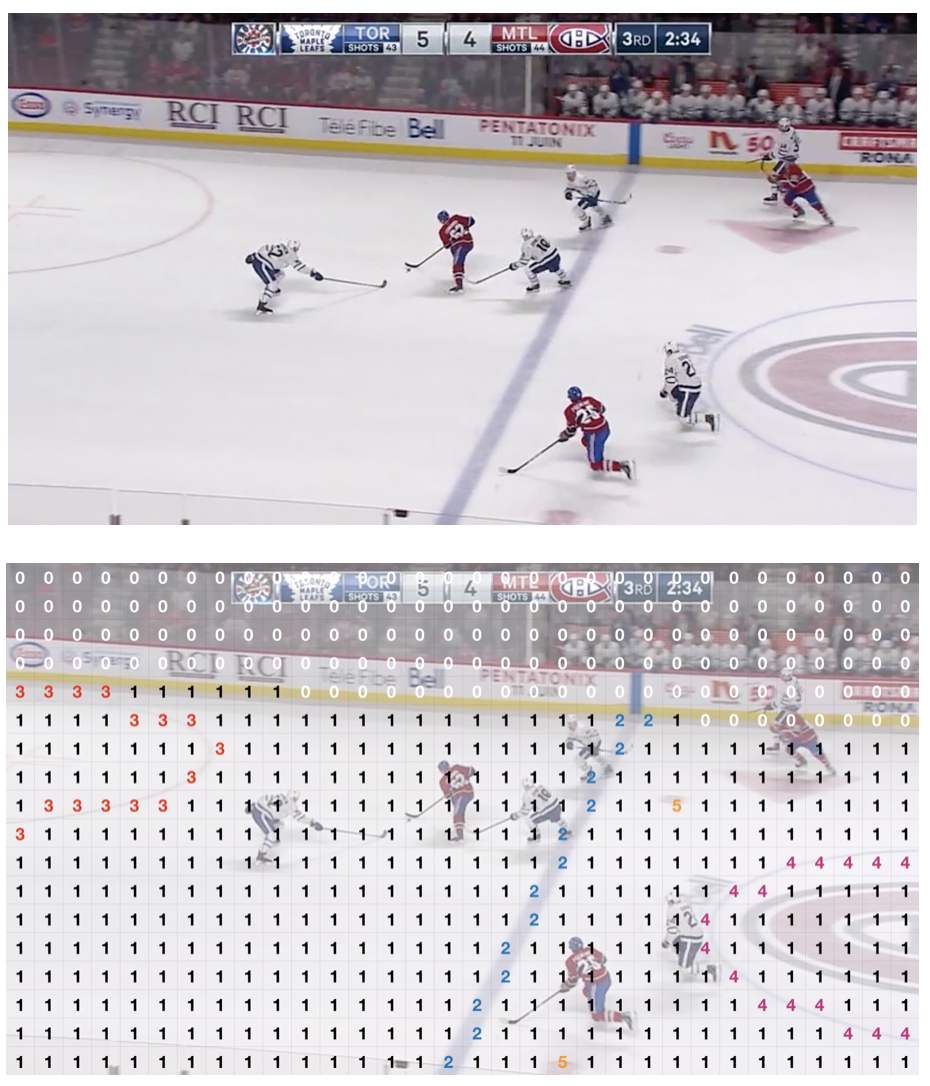
\includegraphics[width=5.5cm, height=5cm]{figures/mask-example.png}
	\caption{Example of mask where each pixel of an image is associated with one class.}
	\label{fig:mask}
\end{figure}

\subsection{Complete workflow}
Once we have a class to every pixel, we now have the output we would like our model to predict. Similarly to other multiclass learning problems, we will have to \textit{one-hot encode} the output of the model so that the output for every pixel will be a vector with the same length as the number of classes. If we look at it matrix-wise instead of pixel-wise, we can say that we will have \textit{one-hot encoded matrix} as the output of the model. Each of those matrix. have the same width and height as the input image, will be related to a specific class and the values predicted by the model will correspond to probabilities to be part of that class.

\begin{figure}[H]
	\centering
	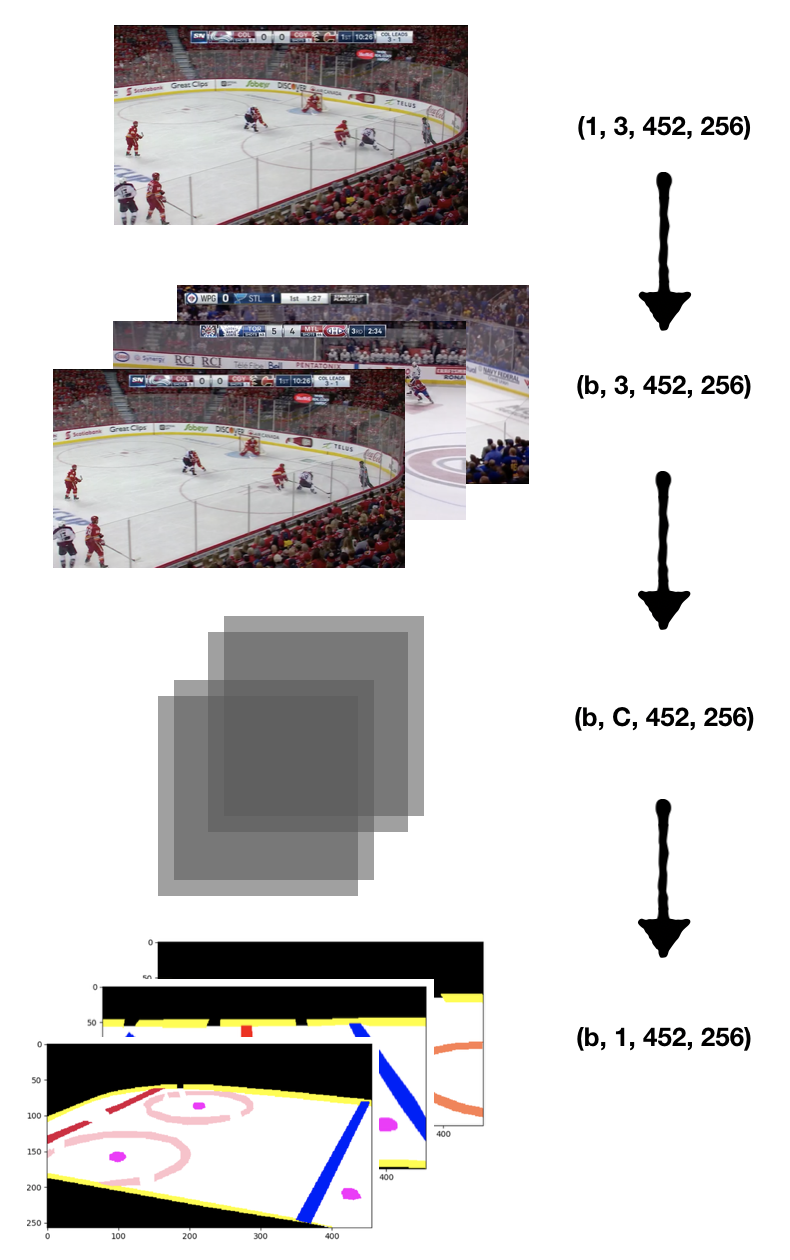
\includegraphics[width=5.5cm, height=10cm]{figures/workflow-dimensions.png}
	\caption{Summary of the workflow behind the semantic segmentation learning task.}
	\label{fig:workflow}
\end{figure}

The figure \ref{fig:workflow} summarizes this workflow where we start from multiple images and ends up with multiple predictions. As such, we start with one RGB image, then we have b images inside one minibatch. At the end of the model, each of those images are \textit{one-hot} encoded to C dimensions, corresponding to the number of classes to predict. Finally, we apply a \texttt{softmax} or any other function that select a predicted class, so that we no longer have C dimensions, but only 1.



\section{Methodology}
\textbf{\label{sec:methodology}}
\begin{itemize}
	\item Semantic segmentation (architerures, loss, data aug)
	\item mapping (plus short)
\end{itemize}


\section{Dataset}
\textbf{\label{sec:dataset}}
\subsection{Dataset creation}
We applied the methodology described earlier to hockey broadcast images. We generated our dataset, which contains images (inputs) and masks (outputs), by ourselves. To do so, we annotated a total of 43 NHL broadcast images. For the annotation part, we used an open source tool called \href{https://github.com/opencv/cvat}{cvat tool}. That tool allowed us to draw polygons around our labels and then associate a class to each pixels in the image.

To choose our labels, we used an iterative approach where we first used our judgment to decide arbitrary categories (ex: ice, crowd, corners, horizontal lines, vertical lines). After that, we used one single image and tried to fit a model using those labels. We then noticed the bahviour of the model regarding those categories and adapted them. For example, we noticed the corners, the horizontal and vertical lines such as the board were difficult to distinguish for the model. As such, we decided to merge them and use one single category called "board". Here are the \textbf{9 categories} we selected at the end: ice, boards, crowd, red line, blue lines, goal lines, circles in end zone, circles in neutral zone and dots. The figure \ref{fig:labeling} is an example of image we extracted and then labeled using our 9 categories.

\begin{figure}[H]
	\centering
	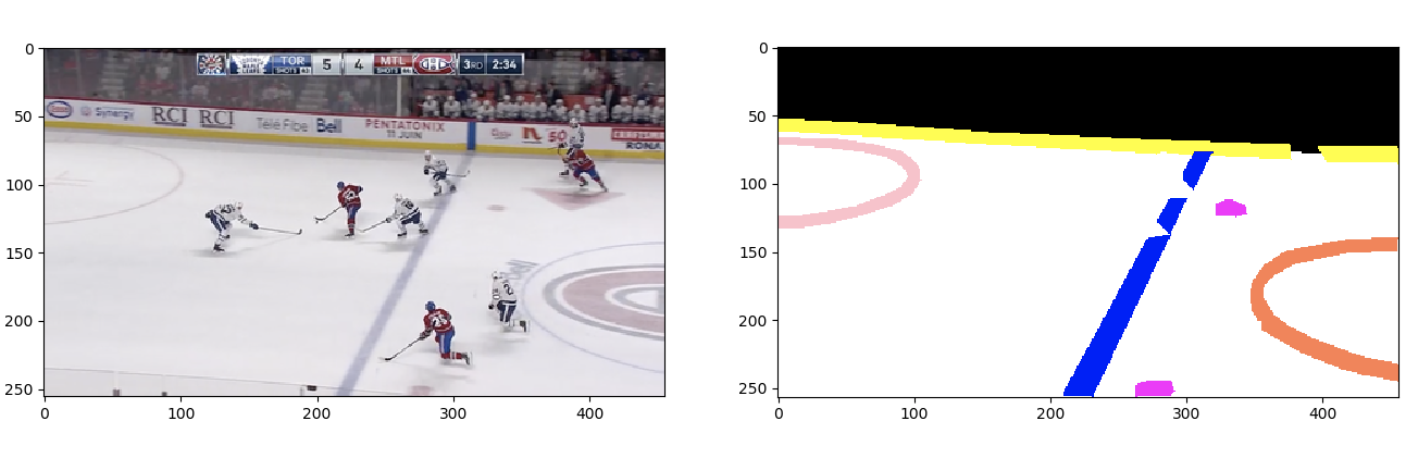
\includegraphics[width=8cm, height=4cm]{figures/labeling-example.png}
	\caption{Example of extracted image (left) and the labeling output (right) using the 9 categories.}
	\label{fig:labeling}
\end{figure}

In the methodology section, we mentionned we had a class imbalance problem. In that section, we tackled this problem by adapting the loss. In the labeling task, we also tackled that class imbalance problem by subjectively drawing larger polygons for rare categories such as dots or circles.



\section{Results}
\textbf{\label{sec:results}}
With the two neural network architectures, the two loss function, our dataset and all the hyperparameters, we achieve to obtain result that we found good for our little dataset. 

\subsection{Hyperparameters}

To find the hyperparameters that gave the best images predictions on the test set, we did a grid search with a lot of check on the prediction by looking at the image. Our best result was achieve with the adapatation of the pretrained VGG 16. For the optimizer, we choose the stochastique gradient descent with a momentum of 0.9 and a small weight decay. The learning rate started at 0.001 and we decreased when the loss was not decreasing anymore. The batch size was 4, the dice loss was used, the image was normalize using the normalization of imagenet and we did 20 epochs. Here is the result that we gathered from our best experiments.
\vspace{2mm}
\setlength{\tabcolsep}{1mm}
\begin{tabular}{c c c c c}
	\toprule
	Model & Epochs & Loss & Train Loss & Valid Loss \\
	\midrule
	U-Net & 50 & Dice & 0.8263 & 0.8393 \\
	VGG16 & 20 & Dice & 0.8387 & 0.8023 \\
\end{tabular}

\vspace{1mm}

 Here is sample that shows our best results for VGG16 model on test set images:

\vspace{1mm}
\begin{center}
	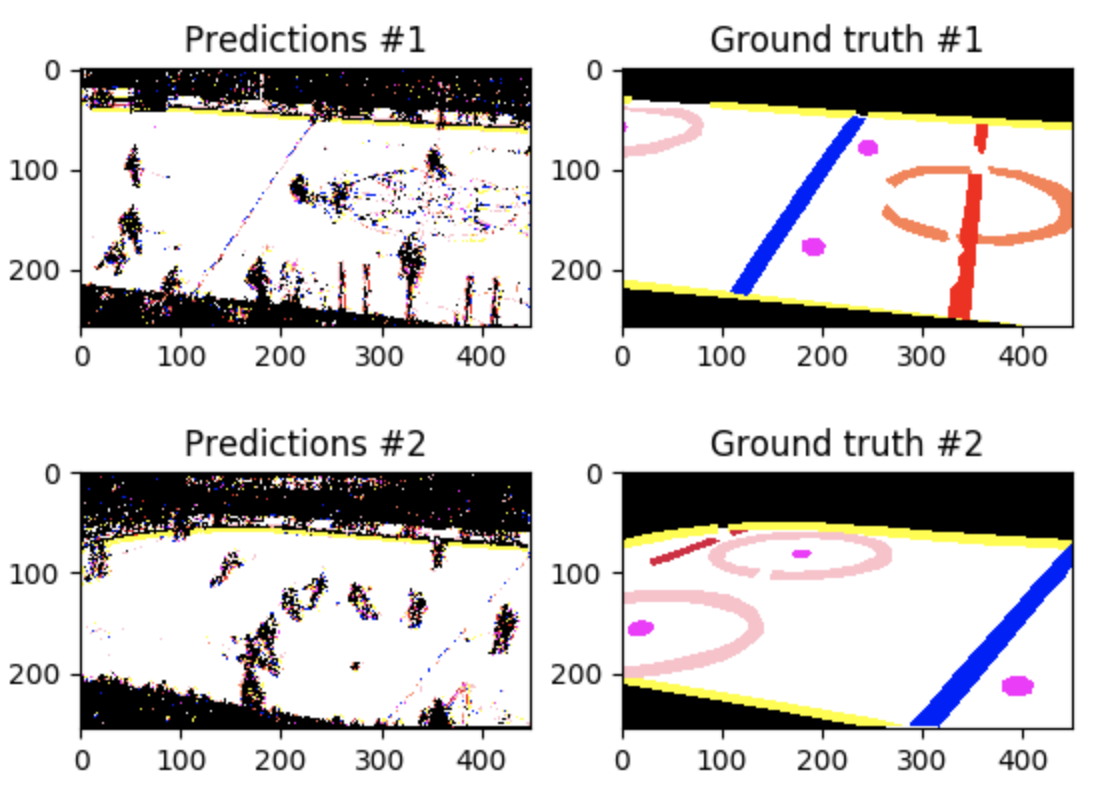
\includegraphics[width=7.5cm,height=4.86cm]{figures/test-9-class.png}
\end{center}

We see that the upper board seems to be well predicted. The player on the ice are labelled as crowd, but it's not supprising since the player on the beach and the crowd are labbeled as crowd. The line appears a little bit.



\section{Conclusion}
\textbf{\label{sec:conclusion}}
In conclusion, we can first say that we need more images. The lack of images is even more problematic for a non pre-trained model such as the U-Net model. We can also say that a pre-trained model seems to be a must in our learning task, even if we could have a larger dataset. After a lot of training attempts, we also noticed that those can of models seems to learn slowly and over a long period of time. \\
The next steps would be to extract more images. Also, because the pre-trained model was quite successful, we may need to put more focus on using a more specific encoder for that task. In the same idea, we may need to put more efforts on the decoder part of the model, which can hardly be pre-trained in our case. Finally, if we are able to build a adequate semantic segmentation model, we could then use that model to map our images into a 2 dimensional plan.



\bibliographystyle{apacite}

\setlength{\bibleftmargin}{.125in}
\setlength{\bibindent}{-\bibleftmargin}

\bibliography{bibliography}

\end{multicols}

\end{document}